\documentclass[a4paper,10pt]{report}


\usepackage{amsmath}
\usepackage{amssymb}
\usepackage{graphicx}
\usepackage{makeidx}
\usepackage{fancybox}

% Title Page
\title{Kinetic Waves in Plasma}
\author{Thomas Oswald}


\begin{document}

\maketitle
\tableofcontents

\begin{abstract}
\paragraph*{}
This report is part of the course ,,Plasmatheory: Waves and Instabilities'' held by Prof. H. Biernat at the University of Graz. Its subject is the basic elements of kinetic plasma theory and kinetic plasma waves.


\paragraph*{}
In this report, I will start by revising the basics of the kinetic plasma theory. Then I will proceed by deriving the electrostatic waves and discuss Landau damping.
\end{abstract}


\section{Basics of the kinetic plasma theory}
\subsection{Exact phase space}


\paragraph*{}
A plasma consists of many particles of different kind, interacting with each other. Each particle is fully defined by its charge, mass, position vector $\mathbf{q}$ and momentum vector $\mathbf{p}$. When a different set of equations is used for each species, there are two possibilities how to represent the plasma system. The way, I will use, is a 6 dimensional phase space, where each particle is represented by a point. The other possibility is to use a 6N space, where N is the number of particles of this species. Then the momentary state of the system is represented by a single point. The whole procedure, I describe is derived in a more detailed way in \cite{baumjohann1}.

\paragraph*{}
When using the 6 dimensional representation, the exact number density of a particle can be written as

\begin{equation}\label{exact_number_density_one_particle}
    f_{exact,i}(\mathbf{q,p},t)=\delta(\mathbf{q}-\mathbf{q}_i(t))\delta(\mathbf{p}-\mathbf{p}_i(t))
\end{equation}

\paragraph*{}
So the whole exact number density is

\begin{equation}\label{exact_number_density}
    f_{exact}(\mathbf{q,p},t)=\sum_i \delta(\mathbf{q}-\mathbf{q}_i(t))\delta(\mathbf{p}-\mathbf{p}_i(t))
\end{equation}

\paragraph*{}
If the total number of particles is taken to be constant, we can say that a volume in the phase space, dV does not change its size during its evolvement in time, but merely changes its shape. So we can write

\begin{equation}\label{erhaltung_exact_number_density}
    \frac{D}{Dt}f_{exact}(\mathbf{q,p},t)=\left( \frac{\partial}{\partial t} + \mathbf{v}\cdot \nabla_q+\frac{\partial \mathbf{p}}{\partial t}\cdot\nabla_p \right) f_{exact}(\mathbf{q,p},t)=0
\end{equation}

\paragraph*{}
$\frac{D}{Dt}$ is the substantial derivative. $\frac{\partial \mathbf{p}}{\partial t}$ is the force, which is $q(\mathbf{E}+\mathbf{v}\times \mathbf{B})$ in our case, so

\begin{equation}\label{Klimontovich-Dupree}
    \left( \frac{\partial}{\partial t} + \mathbf{v}\cdot \nabla_q+q(\mathbf{E}_m+\mathbf{v}\times \mathbf{B}_m)\cdot\nabla_p \right) f_{exact}(\mathbf{q,p},t)=0
\end{equation}

\paragraph*{}
This important equation is called the \emph{Klimontovich-Dupree equation}. Subscript m indicates that the microscopic fields are meant.

\subsection{The average Distribution function}
\paragraph*{}
We define the averaged phase space density.

\begin{equation}\label{f_av}
    f=\langle f_{exact}(\mathbf{q,p},t) \rangle
\end{equation}

\paragraph*{}
So the exact phase state density consists of two parts, the averaged phase space density and a fluctuation term.

\begin{equation}\label{f_exact}
    f_{exact}=f+ \delta f_{exact}(\mathbf{q,p},t)
\end{equation}

\paragraph*{}
$\langle \delta f_{exact}(\mathbf{q,p},t) \rangle =0$ must be true. Similar

\begin{eqnarray}
% \nonumber to remove numbering (before each equation)
  \mathbf{E}_m(\mathbf{q,p},t) &=& \mathbf{E}(\mathbf{q,p},t)+\delta \mathbf{E}(\mathbf{q,p},t) \\
 \mathbf{B}_m (\mathbf{q,p},t)&=& \mathbf{B}(\mathbf{q,p},t)+\delta \mathbf{B}(\mathbf{q,p},t) \\
\langle \delta \mathbf{E}(\mathbf{q,p},t) \rangle &=& 0 \\
\langle \delta \mathbf{B}(\mathbf{q,p},t) \rangle &=& 0\end{eqnarray}

\paragraph*{}
Inserting these equations into (\ref{Klimontovich-Dupree}) yields the kinetic equation.

\begin{equation}\label{kinetic_equation}
    \left( \frac{\partial}{\partial t} + \mathbf{v}\cdot \nabla_q+q(\mathbf{E}+\mathbf{v}\times \mathbf{B})\cdot\nabla_p \right) f(\mathbf{q,p},t)+ q(\mathbf{\delta E}+\mathbf{v}\times \mathbf{\delta B})\cdot\nabla_p \delta f(\mathbf{q,p},t)=0
\end{equation}

\paragraph*{}
It describes the evolution of the coarse grained phase state density under influence of the averaged fields. The value of the distribution function f can be interpreted as the probability to find a particle in the volume d\textbf{q}d\textbf{p} of the phase space. The last term models the interaction between fields and particles. When collisions between particles are to be considered, there might be additional terms. Space plasma can be regarded as collision less most of the time, so I will neglect the collision term and even the EM interaction term in equation (\ref{kinetic_equation}). Then I get the simplest kinetic equation that can be used to describe plasma, the Vlasov equation.

\begin{equation}\label{vlasov1}
    \left( \frac{\partial}{\partial t} + \mathbf{v}\cdot \nabla_q+q(\mathbf{E}+\mathbf{v}\times \mathbf{B})\cdot\nabla_p \right) f(\mathbf{q,p},t) =0
\end{equation}

\paragraph*{}
This equation can also be written in a slightly different form, where index e describes the distribution function for the electrons, i for the ions.

\begin{eqnarray}
% \nonumber to remove numbering (before each equation)
  \left( \frac{\partial}{\partial t} + \mathbf{v_e}\cdot \nabla_q-\frac{e}{m_e}(\mathbf{E}+\mathbf{v_e}\times \mathbf{B})\cdot\nabla_v \right) f_e(\mathbf{q,v},t) &=& 0 \label{vlasov_e}\\
\left( \frac{\partial}{\partial t} + \mathbf{v_i}\cdot \nabla_q+\frac{Ze}{m_i}(\mathbf{E}+\mathbf{v_i}\times \mathbf{B})\cdot\nabla_v \right) f_i(\mathbf{q,v},t) &=& 0\label{vlasov_i}\end{eqnarray}

\paragraph*{}
These equations can be manipulated in a way to produce the equations of the two fluid theory, as shown in \cite{kippenhahn}, so two fluid theory is a subset of the kinetic theory.

\subsection{The Liouville theorem}
\paragraph*{}
If collisions and interactions between particles and microscopic fields can be neglected, such that $\nabla \cdot \mathbf{v}=0$, as in case of Vlasov's equation, Liouville's theorem holds, which states that a phase space volume does not change, it marly can be deformed. This is a result of the conservation of particle numbers, so it holds exactly only for exact phase state density. In averaged phase space, it is only an approximation, although normally a good one.

\paragraph*{}
A volume in phase space $dV$ moves under the action of the Lorenz force like an incompressible fluid. The reason for this behavior is that the divergency of the velocity is zero.

\subsection{The macroscopic observables}
To get macroscopic observables, which do not depend on the velocity distribution but are the result of it, one has to take the respective velocity moment of the distribution, that is, integrate over the velocity space to get rid of the velocity dependance.

\begin{equation}\label{velocity_moment_allgemein}
    M_i(\mathbf{q},t)=\int \mathbf{v}^i f(\mathbf{q,v},t)d^3v
\end{equation}

$\mathbf{v}^i$ is the dyadic product of the velocity vector with itself, i times. The first four moments are the interesting ones. When we integrate the distribution function over the whole phase space we get the number of particles:

\begin{equation}\label{particle number}
    N(\mathbf{q,v},t)=\int_V \int_v f(\mathbf{q,v},t)d^3v d^3q
\end{equation}

When You divide this n umber by the volume, You get the number density:

\begin{equation}\label{velocity_moment_number_density}
    n(\mathbf{q},t)=\int f(\mathbf{q,v},t)d^3v
\end{equation}


Then the bulk velocity,

\begin{equation}\label{velocity_moment_bulc_velocity}
    \mathbf{v}_b(\mathbf{q},t)=\frac{1}{n}\int \mathbf{v} f(\mathbf{q,v},t)d^3v
\end{equation}


the pressure tensor, where we integrate over the velocity fluctuations

\begin{equation}\label{velocity_moment_pressure}
    \mathbf{P}(\mathbf{q},t)=m\int (\mathbf{v}-\mathbf{v}_b)^2 f(\mathbf{q,v},t)d^3v
\end{equation}


and the heat tensor.

\begin{equation}\label{velocity_moment_heat_tensor}
    \mathbf{Q}(\mathbf{q},t)=m\int (\mathbf{v}-\mathbf{v}_b)^3 f(\mathbf{q,v},t)d^3v
\end{equation}

\paragraph*{}
the trace of the heat tensor corresponds to the heat flux vector.

\begin{equation}\label{heat_flux}
    \mathbf{\phi}_H(\mathbf{q},t)=\frac{1}{2} m\int (\mathbf{v}-\mathbf{v}_b)\cdot(\mathbf{v}-\mathbf{v}_b)^2 f(\mathbf{q,v},t)d^3v
\end{equation}

\paragraph*{}
the trace of the pressure tensor, which corresponds tho the isotropic part of the pressure, called thermal pressure, can be used to define to a scalar temperature of the plasma component, which is called kinetic temperature.

\begin{equation}\label{kinetic_temperature}
    T(\mathbf{q},t)=\frac{m}{2kn}\int (\mathbf{v}-\mathbf{v}_b) \cdot (\mathbf{v}-\mathbf{v}_b) f(\mathbf{q,v},t)d^3v
\end{equation}

\paragraph*{}
This temperature is not the same as the thermodynamic temperature which is defined only for a system in equilibrium. The kinetic temperature is a directed parameter. In an anisotropic plasma, it has different values for different directions, because the velocity distributions differ.


\section{Kinetic plasma waves}

\subsection{Electrostatic waves}
\paragraph*{}
Treating the electrostatic waves by a kinematic approach results in more information than by other theories. In particular I will show that there is a damping mechanism intrinsic in the theory. This mechanism, called Landau Damping, is not explained by other methods.

\paragraph*{}
For simplicity, I will look at a quasi-neutral plasma, where the ions are static, so I will only use the equation for the electron gas (\ref{vlasov_e}) without the subscript e.

\begin{equation}
    \left( \frac{\partial}{\partial t} + \mathbf{v}\cdot \nabla_q-\frac{e}{m}(\mathbf{E}+\mathbf{v}\times \mathbf{B})\cdot\nabla_v \right) f(\mathbf{q,v},t) = 0
\end{equation}

A useful approach is the variational principle, so we disturb the fields.

\begin{eqnarray}
% \nonumber to remove numbering (before each equation)
  f &=& f_0+f_1 \\
\mathbf{E} &=& \mathbf{E}_0+\mathbf{E}_1 \\
\mathbf{B} &=& \mathbf{B}_0+\mathbf{B}_1\end{eqnarray}

\paragraph*{}
We neglect any background field ($\mathbf{E}_0=\mathbf{B}_0=0$) and regard the undisturbed density function as constant, such that any derivative is vanishing. Further we say that there is no current in the undisturbed plasma.

\begin{equation}
    \mathbf{v}_{b,0}=\frac{1}{n_0}\int{f_0\mathbf{v}d^3p}=0
\end{equation}

\paragraph*{}
The electrons must have a velocity distribution such that  $f(\textbf{v)}\rightarrow 0$ as $v\rightarrow \infty$. When we consider only terms to order 1, we get

\begin{equation}
 \frac{\partial f_1}{\partial t} + (\mathbf{v}\cdot \nabla_q) f_1-\left( \frac{e}{m}(\mathbf{E}_1+\mathbf{v}\times \mathbf{B}_1)\cdot\nabla_v \right) f_0 = 0
\end{equation}

\paragraph*{}
If the variation takes place only in one direction, the rotational term must vanish and we only have to take into account die component in which the disturbance takes place, say the x axis. So we get a scalar equation.

\begin{equation}
 \frac{\partial f_1}{\partial t} + \left( v \frac{\partial }{\partial x} \right) f_1 =  \frac{e}{m}E_1 \cdot \frac{\partial}{\partial v}  f_0
\end{equation}

\paragraph*{}
I omitted the subscript for shorter notation. Now we postulate a sinusoidal distribution of the fields:

\begin{eqnarray}
% \nonumber to remove numbering (before each equation)
  f_1 &=& f e^{i(kx-\omega t)} \\
f_0 &=& f_0(v) \\
E_1 &=& E e^{i(kx-\omega t)}
\end{eqnarray}

\paragraph*{}
 E is the disturbance amplitude of the electric field. It shall be constant. Hence we get

\begin{equation}
 \frac{\partial }{\partial t} f e^{i(kx-\omega t)} + \left( v \frac{\partial }{\partial x} \right) f e^{i(kx-\omega t)}= \left( \frac{e}{m} E e^{i(kx-\omega t)}\frac{\partial}{\partial v} \right) f_0
\end{equation}

\paragraph*{}
and

\begin{equation}\label{de1}
 -i \omega f  +  ikv  f = \frac{e}{m} E \frac{\partial}{\partial v}  f_0
\end{equation}

\paragraph*{}
So we have one relation between the disturbance amplitudes E and f. \footnote{I want to emphasize that this equation is not completely valid in a physical sense. We did perform a fourier transform in both, space and time, which presumes spatially and temporally periodically varying parameters. While the former can be justified, this is not necessarily true for the temporal periodicity. There exists a derivation where the transform with respect to time is not performed, but it is mathematically more demanding. It uses a Laplace transform with respect to time, instead of the second Fourier transform.}The second one we get from one of the Maxwell equations.

\begin{equation}\label{coloumb}
    \nabla \cdot \mathbf{E} = \frac{\varrho_e}{\epsilon_0}
\end{equation}

\paragraph*{}
or for our one dimensional case:

\begin{equation}\label{coloumb_1D}
     i k E e^{i(kx-\omega t)} = \frac{\varrho_e}{\epsilon_0}
\end{equation}

\paragraph*{}
$\varrho_e$ is the charge density which can be written as

\begin{eqnarray}
% \nonumber to remove numbering (before each equation)
  \varrho_e &=& eZn_i -en_e \\
 &=& eZn_i-e \int^{\infty}_{-\infty }{(f_0+f_1)dv}
 \end{eqnarray}

But in case of quasi neutrality, this entity must be zero for the undisturbed case:

\begin{equation}
    eZn_i-e \int^{\infty}_{-\infty }{f_0 dv}=0
\end{equation}

So

\begin{equation}
    \varrho_e = e \int^{\infty}_{-\infty }{f e^{i(kx-\omega t)} dv}
\end{equation}

By substituting this into equation (\ref{coloumb_1D}) and dividing by the exponential term, we get

\begin{equation}\label{coloumb_1D_2}
    i k E = \frac{1}{\epsilon_0} e \int^{\infty}_{-\infty } {f  dv}
\end{equation}

Now we can isolate $f$ in equation (\ref{de1}) and substitute it into (\ref{coloumb_1D_2}).

\begin{equation}
       f = -i\frac{e}{m k} E \frac{\frac{\partial f_0}{\partial v}}{v-\frac{\omega}{k}}
\end{equation}

\begin{equation}\label{dispersion_relation}
 \frac{e^2}{\epsilon_0 k^2 m}  \int^{\infty}_{-\infty }{  \frac{\frac{\partial f_0}{\partial v}}{v-\frac{\omega}{k}} dv} =1
\end{equation}

\paragraph*{}
This is the dispersion relation for an electrostatic wave without magnetic field. We define

\begin{equation}
    n_0= \int^{\infty}_{-\infty }{f_0 dv}
\end{equation}

and

\begin{equation}
    F(v)=\frac{f_0(v)}{n_0}
\end{equation}

such that

\begin{equation}
     \int^{\infty}_{-\infty }{F dv}=1
\end{equation}

Hence

\begin{equation}\label{dispersion_relation1}
 \frac{e^2}{\epsilon_0 k^2 m}  \int^{\infty}_{-\infty }{  \frac{n_0\frac{\partial F}{\partial v}}{v-\frac{\omega}{k}} dv} =1
\end{equation}

and

\begin{equation}
    \omega_p^2=\frac{n_0 e^2 }{m \epsilon_0}
\end{equation}

then

\begin{equation}\label{dispersion_relation2}
 \frac{ \omega_p^2}{ k^2}  \int^{\infty}_{-\infty }{  \frac{\frac{\partial F}{\partial v}}{v-\frac{\omega}{k}} dv} =1
\end{equation}

When comparing this equation with the respective dispersion relation of two component theory, one notes several points:

\begin{itemize}
    \item The result of the dispersion relation depends now on the distribution function. It can be shown that the dispersion relations are equivalent, when postulating a Maxwell distribution of velocities.
\item There are also solutions for a complex $\omega$.
\item A complex $\omega$ leads to damping.
\end{itemize}

The last item will be treated in the next subsection.

\subsection{Landau damping}

The dispersion relation (\ref{dispersion_relation2}) can result in a complex $\omega$, which, in turn, leads to waves that are either damped or excited. The imaginary part of the frequency is normally small in relation to the real part. This was expected, since, otherwise two fluid theory would not produce realistic predictions, which it does.\\

The important part of the dispersion relation is the integral.

\begin{equation}\label{integral}
    I=\int^{\infty}_{-\infty }{  \frac{\frac{\partial F}{\partial v}}{v-\frac{\omega}{k}} dv}=- \frac{k}{\omega} \int^{\infty}_{-\infty }{  \frac{\frac{\partial F}{\partial v}}{1-\frac{vk}{\omega}} dv}
\end{equation}

The distribution function must tend to zero if the velocity goes to plus or minus infinity. We postulate the maximum at $v=0$ (no bulk velocity), so the shape of $F$ shall be like a Maxwell distribution. Figures \ref{fig_maxwell} and \ref{fig_maxwell_diff} show the plots of the Maxwell distribution function and its derivative. Figure \ref{fig_denominator} shows the denominator of the integral, if $\frac{\omega}{k}=3$.


\begin{figure}
  % Requires \usepackage{graphicx}
  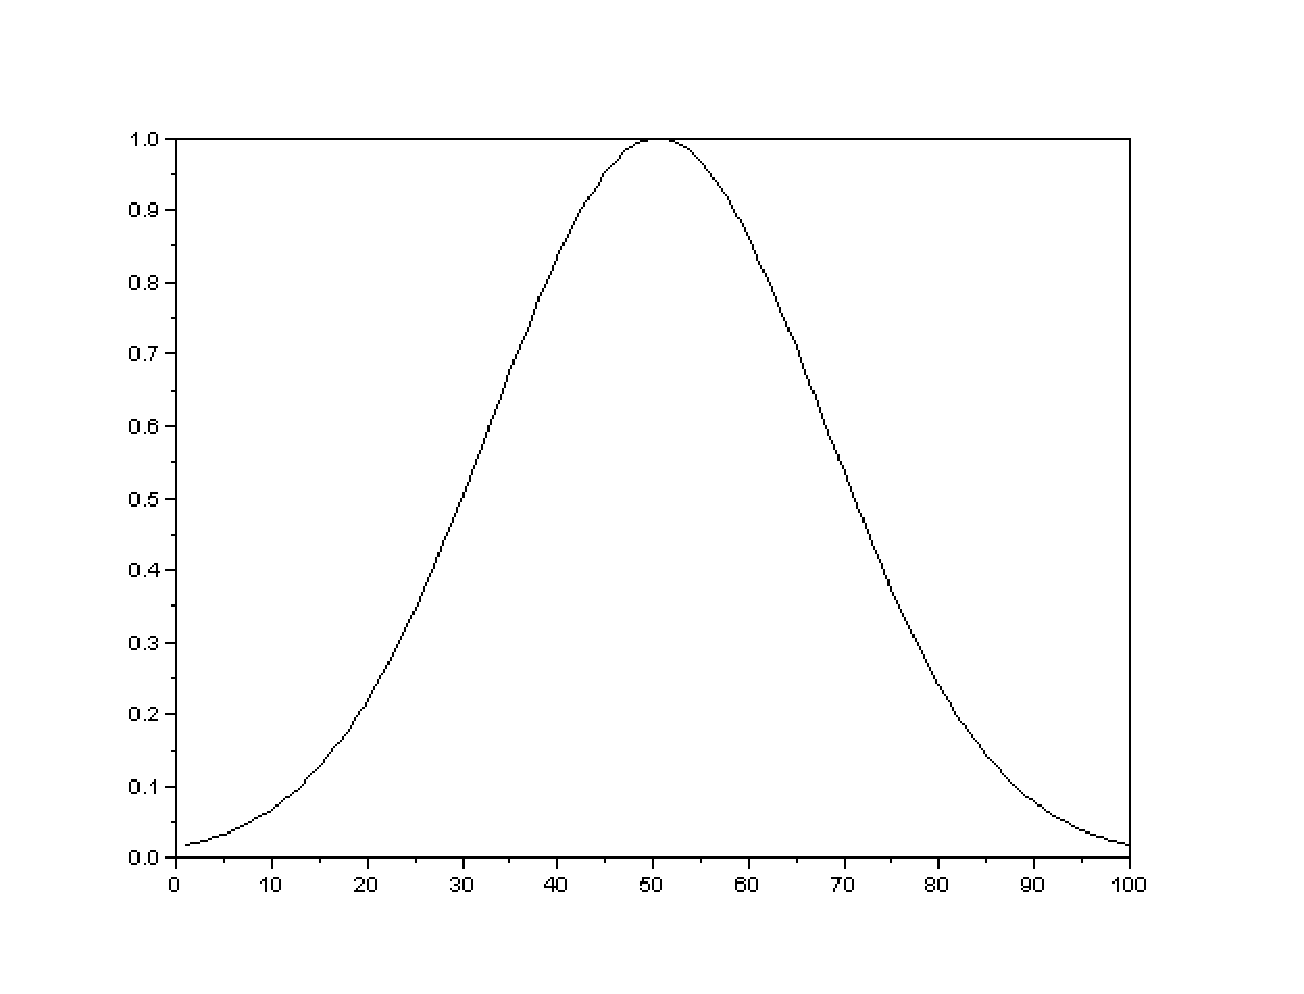
\includegraphics[width=12cm]{maxwell_dist.eps}\\
  \caption{Maxwell Distribution}\label{fig_maxwell}
\end{figure}

\begin{figure}
  % Requires \usepackage{graphicx}
  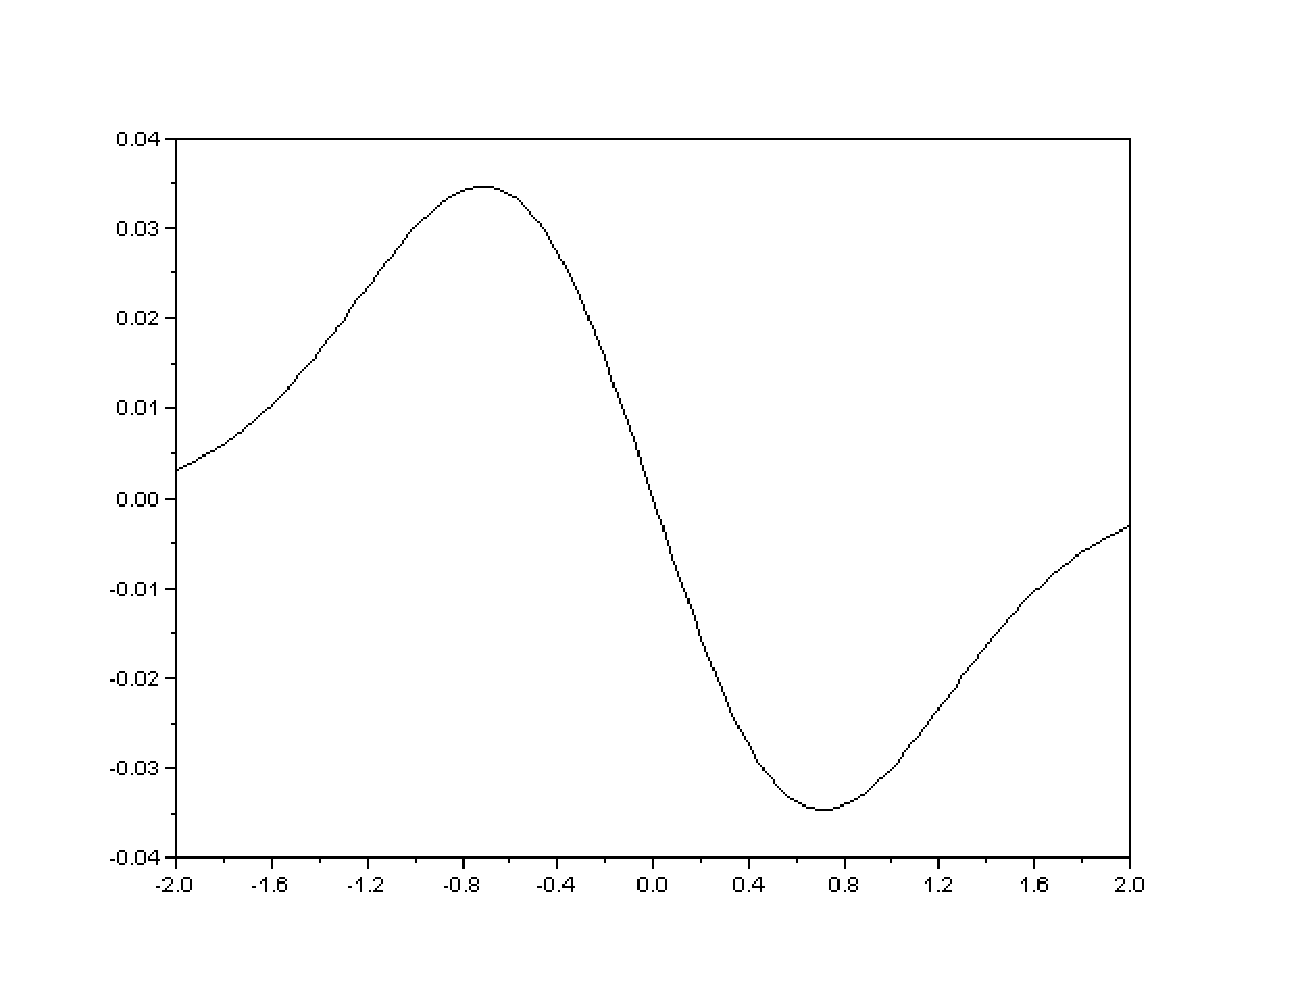
\includegraphics[width=12cm]{maxwell_dist_diff.eps}\\
  \caption{Derivative of Maxwell Distribution}\label{fig_maxwell_diff}
\end{figure}

\begin{figure}
  % Requires \usepackage{graphicx}
  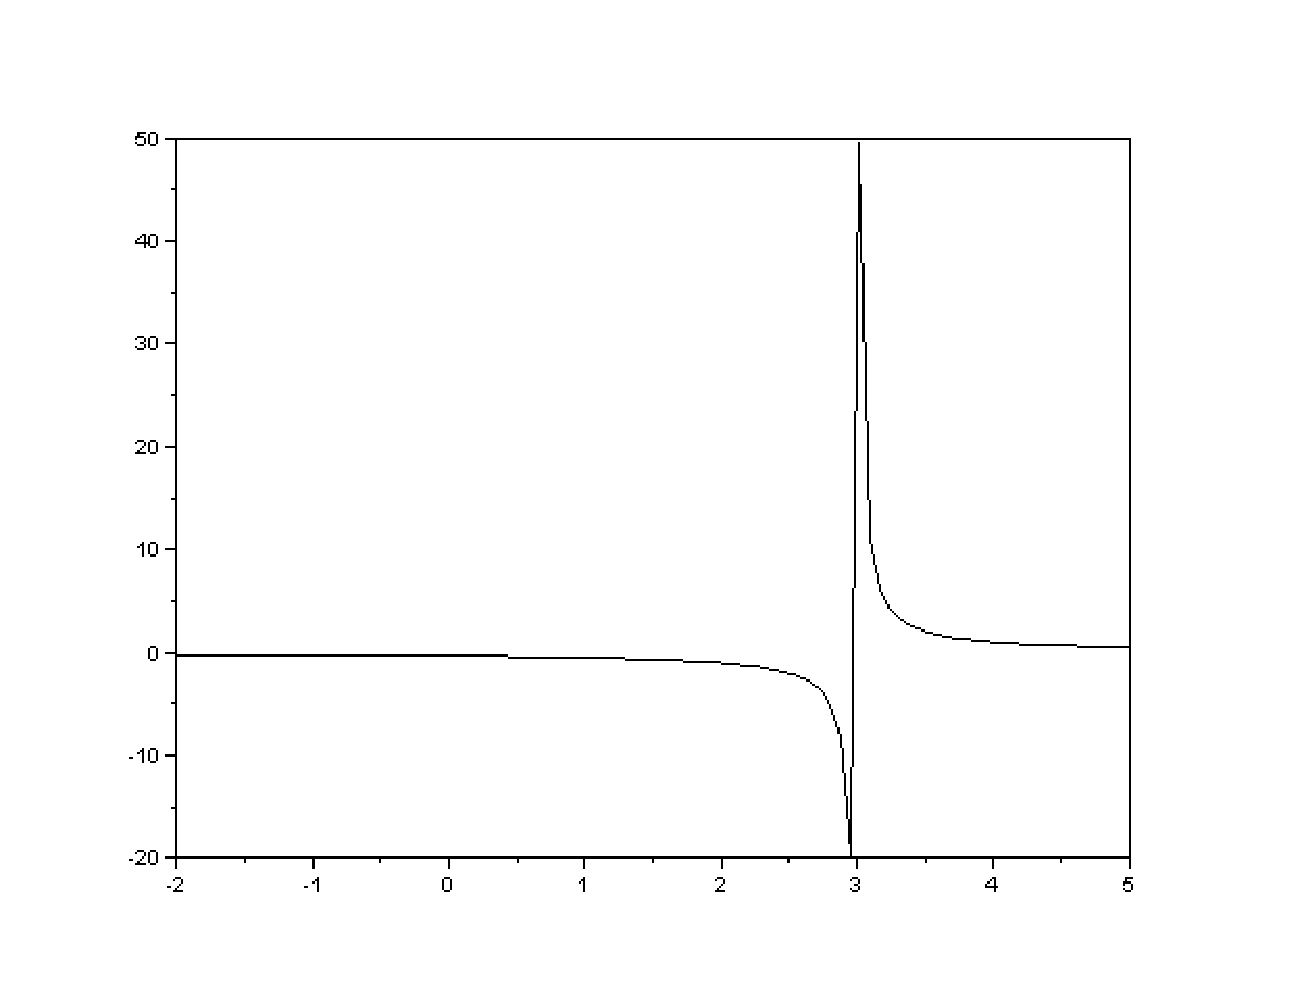
\includegraphics[width=12cm]{nenner.eps}\\
  \caption{Denominator of the integral:omega/k=3}\label{fig_denominator}
\end{figure}

So the numerator and the denominator of the kernel of the integral are prominent in different regions of the range of the velocity, as long as the maximum of F and $\frac{\omega}{k}$ are far enough apart. Then we can divide the integral in two parts, where the boundary is half way between max(v) and $\frac{\omega}{k}$. I call this speed $v_{sep}$.

\begin{eqnarray}
% \nonumber to remove numbering (before each equation)
  I &=& I_1 +I_2 \label{sep_int} \\
I_1 &=& \int^{v_{sep}}_{-\infty }{  \frac{\frac{\partial F}{\partial v}}{v-\frac{\omega}{k}} dv} \\
I_2 &=& \int^{\infty}_{v_{sep} }{  \frac{\frac{\partial F}{\partial v}}{v-\frac{\omega}{k}} dv}\end{eqnarray}

\subsubsection{Ad Integral 1:}

In the part of the region, where the differential of F is prominent, $|\frac{k v}{\omega}|$ is small. Here we can approximate the denominator.

\begin{equation}
\left( 1-\frac{k v}{\omega} \right)^{-1}=1+ \frac{k v}{\omega} + \left( \frac{k v}{\omega} \right)^2 ...
\end{equation}

Hence

\begin{equation}
    I_1=-\frac{k}{\omega} \left( \int^{\infty}_{-\infty } {\frac{\partial F}{\partial v}dv } + \frac{k}{\omega}\int^{\infty}_{-\infty } {\frac{\partial F}{\partial v} v dv }  + \frac{k^2}{\omega^2}\int^{\infty}_{-\infty } {\frac{\partial F}{\partial v} v^2 dv } + ...\right)
\end{equation}

By partial integration one gets

\begin{eqnarray}
    I_1&=&-\frac{k}{\omega} \left[ F \right]^{\infty}_{-\infty } \\
    &-& \frac{k^2}{\omega^2} \left[ F v \right]^{\infty}_{-\infty } +  \frac{k^2}{\omega^2} \int^{\infty}_{-\infty } F dv \nonumber \\
&-& \frac{k^3}{\omega^3} \left[ F v^2 \right]^{\infty}_{-\infty } +  \frac{2 k^3}{\omega^3} \int^{\infty}_{-\infty } Fv dv \nonumber \\
&-& \frac{k^4}{\omega ^4} \left[ F v^3 \right]^{\infty}_{-\infty } +  \frac{3 k^4}{\omega^4} \int^{\infty}_{-\infty } Fv^2 dv - ... \nonumber
\end{eqnarray}

Since F is zero at plus or minus infinity, we can set all negative terms to zero.

\begin{eqnarray}
    I_1&=& \frac{k^2}{\omega^2} \int^{\infty}_{-\infty } F dv  \\
&+& \frac{2 k^3}{\omega^3} \int^{\infty}_{-\infty } Fv dv \nonumber \\
&+&   \frac{2 k^4}{\omega^4} \int^{\infty}_{-\infty } Fv^2 dv + ...\nonumber
\end{eqnarray}

$Fv$ is an even function, so this integral (and all even integrals of higher order) is(are) also zero. The following equation remains.

\begin{eqnarray}
    I_1&=& \frac{k^2}{\omega^2} \int^{\infty}_{-\infty } F dv + \frac{3 k^4}{\omega^4} \int^{\infty}_{-\infty } {Fv^2 dv} + ... \\
&=& \frac{k^2}{\omega^2}  + \frac{3 k^4}{\omega^4} \bar{v^2} + ...\label{result_I1}
\end{eqnarray}

\subsubsection{Ad Integral 2:}
If we look at the diagrams, we realize that $\frac{\partial F}{\partial v}$ does not change its value much near $v=\frac{\omega}{k}$, where the denominator of the kernel is zero. So we take the derivative as a constant and set the integration range from $\frac{\omega}{k}- \left( \frac{\omega}{k}- v_{sep} \right)$ to $\frac{\omega}{k}+\left( \frac{\omega}{k}- v_{sep} \right)$.

\begin{equation}
    I_2= \frac{\partial F}{\partial v}\mid_{v=\frac{\omega}{k}} \int^{2\frac{ \omega}{k} - v_{sep} }_{v_{sep}} {\left( v-\frac{\omega}{k} \right)^{-1} dv }
\end{equation}

Since $\omega$ is in general complex, we can split this integral in its real and imaginary part.

\begin{eqnarray}
  I_3 &=& \int^{2\frac{ \omega}{k} - v_{sep}}_{v_{sep}} {\left( v-\frac{\omega_r}{k} -i\frac{\omega_i}{k}\right)^{-1} dv } \\
 &=& \int^{2\frac{ \omega}{k} - v_{sep}}_{v_{sep}}{\frac{v-\frac{\omega_r}{k}}{\left( v-\frac{\omega_r}{k} \right)^2+\left( \frac{\omega_i}{k} \right)^2} dv } +  \frac{i\omega_i}{k}\int^{2\frac{ \omega}{k} - v_{sep}}_{v_{sep}}{\frac{1}{\left( v-\frac{\omega_r}{k} \right)^2+\left( \frac{\omega_i}{k} \right)^2} dv } \\
 &=& I_r+I_i
 \end{eqnarray}

$I_r$ is even about $v=\frac{\omega}{k}$, so it vanishes. For $I_i$ we substitute $x=v-\frac{\omega_r}{k}$ and get the standard integral

\begin{eqnarray}
    I_i&=&\frac{i\omega_i}{k} \int^{+(\frac{\omega_r}{k}- v_{sep})}_{-(\frac{\omega_r}{k}- v_{sep})}{\frac{1}{x^2+\frac{\omega_i^2}{k^2}}dx} \\
&=& \frac{i\omega_i}{k} \left[ \frac{k}{\omega_i} \arctan{\frac{x}{\frac{\omega_i}{k}}}\right]_{-(\frac{\omega_r}{k}- v_{sep})}^{+(\frac{\omega_r}{k}- v_{sep})} \\
&=& i \left[ \arctan{\frac{x}{\frac{\omega_i}{k}}}\right]_{-(\frac{\omega_r}{k}- v_{sep})}^{+(\frac{\omega_r}{k}- v_{sep})} \\
&=& i \left[ \arctan \left(\frac{+(\frac{\omega_r}{k}- v_{sep})}{\frac{\omega_i}{k}}\right) - \arctan \left( \frac{-(\frac{\omega_r}{k}- v_{sep})}{\frac{\omega_i}{k}}\right) \right]
\end{eqnarray}

Since the real part of the frequency is far greater than the imaginary part, we can extend the boundary of the integral to plus and minus infinity.

\begin{eqnarray}
    I_i&=& i \left[ \arctan {(\infty)} - \arctan {(-\infty)} \right]\\
&=& i \pi
\end{eqnarray}

Hence

\begin{equation}
    I_3=i \pi
\end{equation}

and

\begin{equation}\label{result_I2}
    I_2=i \frac{\partial F}{\partial v}\mid_{v=\frac{\omega}{k}} \pi
\end{equation}

From equations (\ref{dispersion_relation2}), (\ref{result_I1}) and (\ref{result_I2}), we get

\begin{equation}\label{dispersion_relation_solved}
 \frac{ \omega_p^2}{ k^2}  (I_1+I_2) =1
\end{equation}

or

\begin{equation}\label{dispersion_relation_solved_2}
 \frac{ \omega_p^2}{ k^2}  \left[ \left(\frac{k^2}{\omega^2}  + \frac{3 k^4}{\omega^4} \bar{v^2} \right)+ \left(i \frac{\partial F}{\partial v}\mid_{v=\frac{\omega}{k}} \pi \right) \right] =1
\end{equation}

I dismissed all terms of higher order in the solution of $I_2$. To get a valid dispersion relation, we have to isolate $\omega$.

\begin{eqnarray}
\omega^2 &=&  \omega_p^2  \left[ \left( 1  + \frac{3 k^2}{\omega^2} \bar{v^2} \right)+ \frac{\omega^2}{k^2}\left(i \frac{\partial F}{\partial v}\mid_{v=\frac{\omega}{k}} \pi \right) \right]\\
\omega^2 &=& \omega_p^2 + \omega_p^2 \left[ \frac{3 k^2}{\omega^2} \bar{v^2} + \frac{\omega^2}{k^2}\left(i \frac{\partial F}{\partial v}\mid_{v=\frac{\omega}{k}} \pi \right) \right]
\end{eqnarray}

This equation requires a complex $\omega$. As we postulated at the beginning of the derivation, the disturbance is proportional to

\begin{equation}
    e^{-i \omega t}=e^{-i \omega_r t}e^{ \omega_i t}
\end{equation}

So the imaginary part of the frequency controls the excitation or damping of the wave, depending on its sign. Its sign, in turn, depends on the sign of the slope of the distribution function at the point $\frac{\omega}{k}$. In case of a Maxwell distribution, the slope is negative, which corresponds to a damping situation. This damping is called \emph{Landau damping}.

\subsection{Two fluid instability}

\begin{figure}
  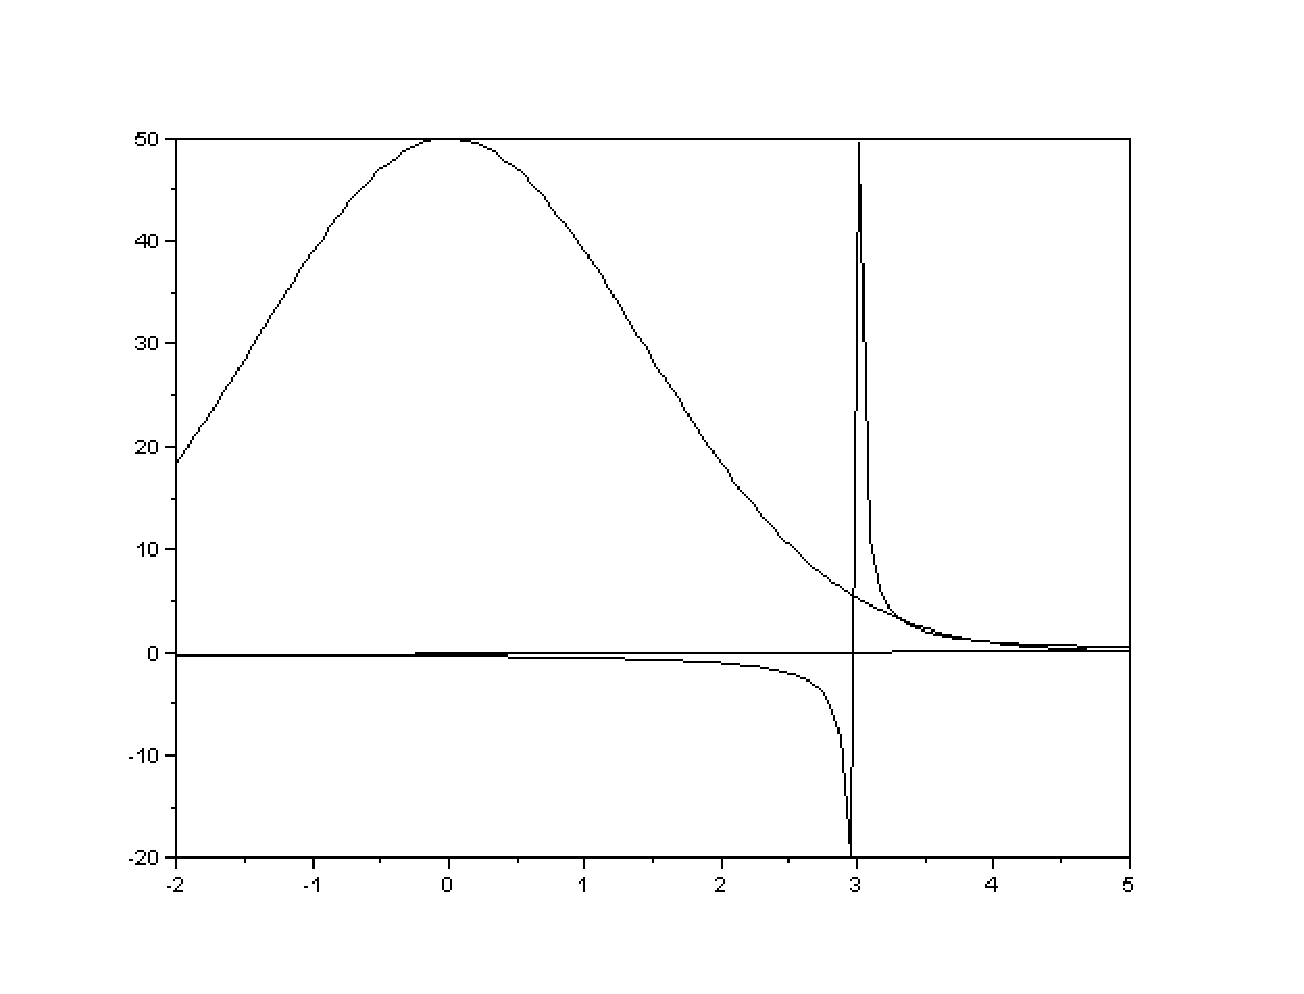
\includegraphics[width=12cm]{maxwell_dist2.eps}\\
  \caption{Maxwell Distribution and the denominator of the integral kernel}\label{fig_maxwell2}
\end{figure}

\begin{figure}
  % Requires \usepackage{graphicx}
  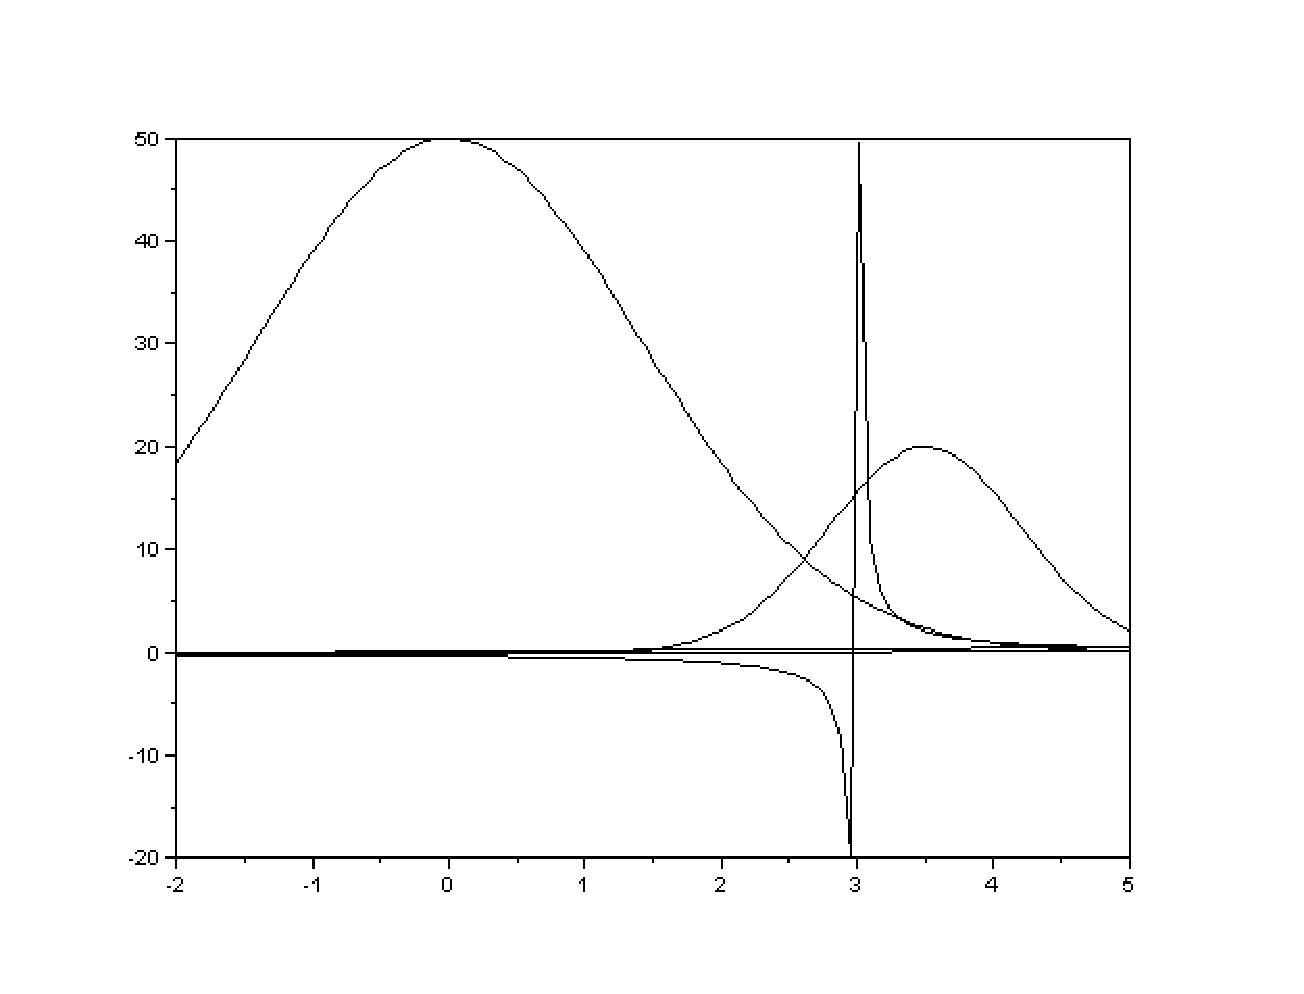
\includegraphics[width=12cm]{twofluids_saperated.eps}\\
  \caption{Maxwell Distribution of two fluids and the denominator of the integral kernel}\label{fig_2fluids_sep}
\end{figure}

\begin{figure}
  % Requires \usepackage{graphicx}
  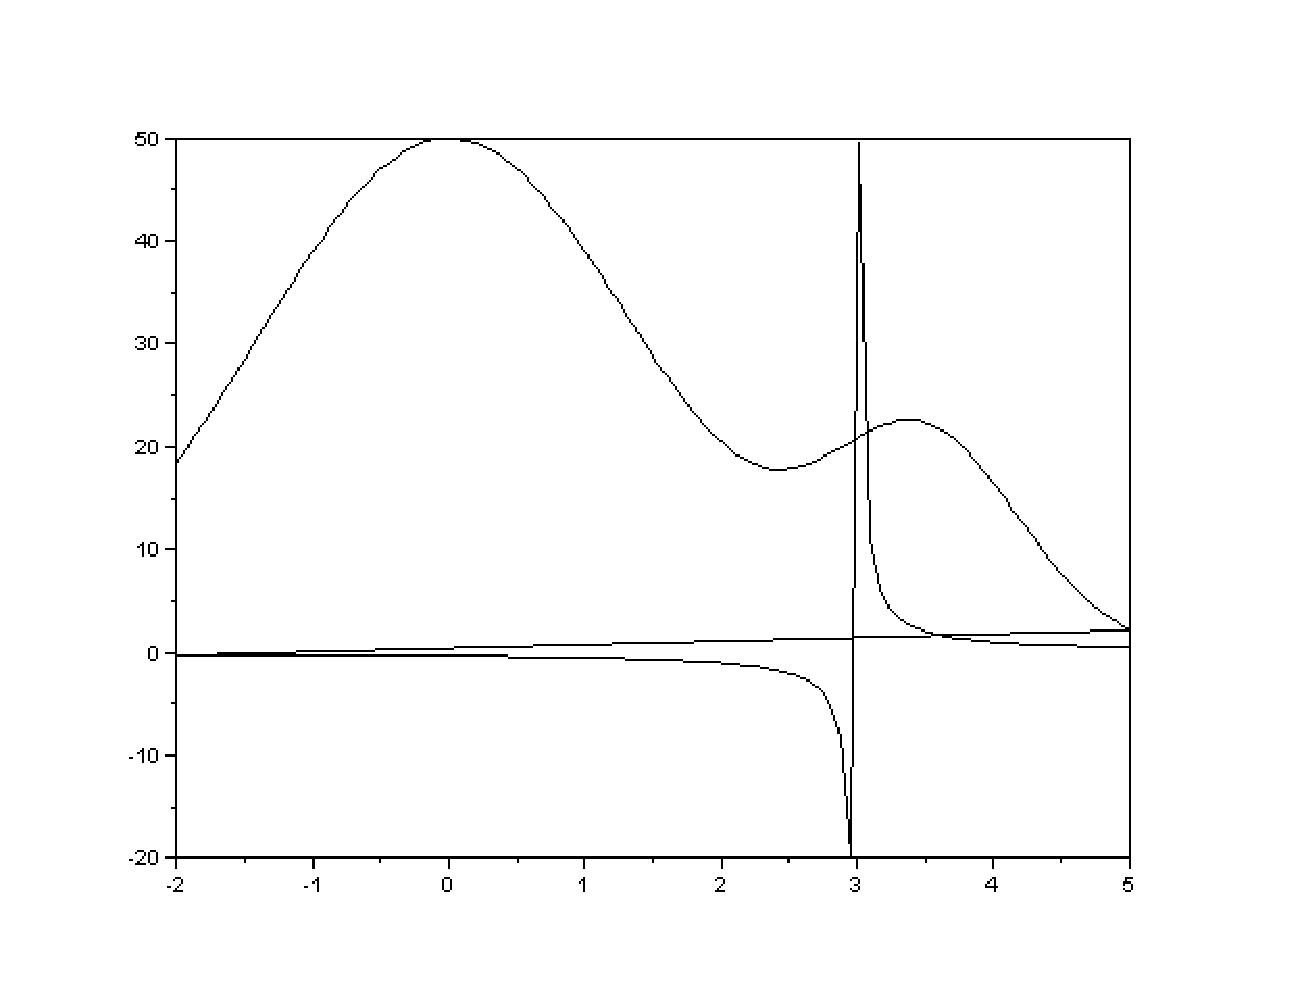
\includegraphics[width=12cm]{twofluids_added.eps}\\
  \caption{Combined Maxwell Distribution of two fluids and the denominator of the integral kernel}\label{fig_2fluids_added}
\end{figure}

As we said in the last subsection, the slope of the velocity distribution function is normally negative, which correspond to damping. But can there be a situation where excitation happens ? The answer is \emph{yes}. I can think of two such situations. The first one is if a second fluid moved through the first one (for instance an electron beam) and has a bulk velocity that is just a little bit greater than $\frac{\omega}{k}$. Then the two distribution functions add, as can be seen in the diagrams \ref{fig_maxwell2} - \ref{fig_2fluids_added}. The slope at the relevant point is now positive.

This is a situation that can not be described by two fluid theory. There is an energy transfer from the electron beam to the underlying fluid, by electrostatic waves, without need of collisions as in normal hydrodynamics.

\subsection{Cyclotron maser Instability}
The second scenario, I want to mention is the cyclotron maser instability. Here, the distribution function is thinned out at the right velocity, because particles with this certain speed are absorbed by a planetary atmosphere. This may happen when particles are trapped in the radiation belt of the planetary magnetic field.

Particles which have a certain velocity component along the magnetic field lines can travel into the high atmosphere of the planet in the auroral region. The probability is high, that they collide with an atmospheric particle, due to the high density in this region. If this happens they are lost for the plasma of the radiation belt, so the distribution function decreases in the opposite direction, where the absorbed particles fail to return after undergoing the mirror process.

\subsection{Qualitative physical description of Landau damping}
\cite{jackson} gives an interesting, physical description of Landau damping. He describes the damping process a result of an energy transfer from the wave to the particles. When the wave is sufficiently slow, particles are trapped in the wave and will move along with the wave. For this to happen, the faster particles have to be slowed down, the particles that are slower than the speed of the wave, are accelerated.

In a normal Maxwell distribution, there are always more slower particles than faster particles, so more particles gain energy than loose energy. This net energy gain is removed from the energy of the wave. It is dampened.

Only when the gradient is reversed, there can be the case that there are more particles around to be slowed down. This would lead to the excitation of the wave.

\bibliography{../Bibliography/MyBib}
\bibliographystyle{geralpha}

\end{document} 